\documentclass{article}
\usepackage[utf8]{inputenc}
\usepackage[T1]{fontenc}
\usepackage{booktabs}
\usepackage{caption}
\usepackage{color}
\usepackage{fancyvrb}
\usepackage{graphicx}
\usepackage{hyperref}
\usepackage{multirow}
\usepackage{parskip}
\usepackage[usenames,dvipsnames]{xcolor}
\usepackage[a4paper, left=3cm, right=3cm, top=3cm, bottom=3cm]{geometry}

\newcommand{\tabitem}{~~\llap{\textbullet}~~}
\def \cmossensoracquisition {\texttt{cmos\_sensor\_acquisition} }
\def \cmossensorinput {\texttt{cmos\_sensor\_input} }
\def \msgdma {\texttt{msgdma} }
\def \dcfifo {\texttt{dc\_fifo} }

\fvset{frame=single,framesep=1mm,numbers=left,framerule=.3mm,numbersep=1mm,commandchars=\\\{\}}

\title{CMOS Sensor Acquisition}
\author{Sahand Kashani}
\date{\today}

\begin{document}

\maketitle

\section{Core Overview}
The \cmossensoracquisition core is a configurable Qsys system that makes it simple to connect a CMOS sensor to a host processor \& memory system.

It combines 3 sub-cores to create a \emph{single}-component CMOS sensor acquisition system easily instantiable in Qsys:

\begin{itemize}
    \itemsep-0.5em
    \item \cmossensorinput
    \item \dcfifo
    \item \msgdma
\end{itemize}

The core comes with a set of C library interfaces that can be used to configure it and start its various operations.

\section{CMOS Sensors}
A CMOS sensor outputs 4 signals with which it is possible to sample its data:
\texttt{
    \begin{itemize}
        \itemsep-0.5em
        \item clock
        \item frame\_valid (1-bit)
        \item line\_valid (1-bit)
        \item data (n-bit)
    \end{itemize}
}

Figure~\ref{fig:cmos_sensor_signals_waveform} shows the relationship between the different signals for 2 frames that contains 2 rows and 3 columns each.

\begin{figure}[h]
    \centering
    \makebox[\textwidth][c]{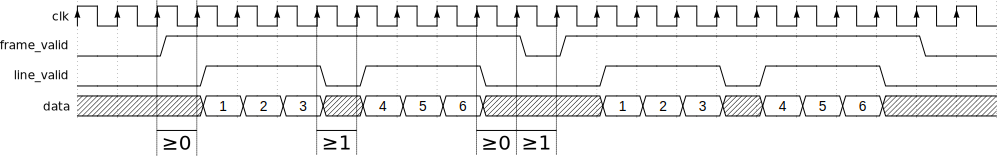
\includegraphics[width=1.0\textwidth]{fig/cmos_sensor_signals_waveform}}%
    \caption{CMOS sensor output signals for two $3\times2$ frames with a pixel depth of 3 bits. Spacing requirements between the various signals are specified in clock cycles.}
    \label{fig:cmos_sensor_signals_waveform}
\end{figure}

\newpage

\section{Block Diagram}
Figure~\ref{fig:block_diagram_internal} shows the connections between the 3 main building blocks that compose the \cmossensoracquisition core.

\begin{figure}[h]
    \centering
    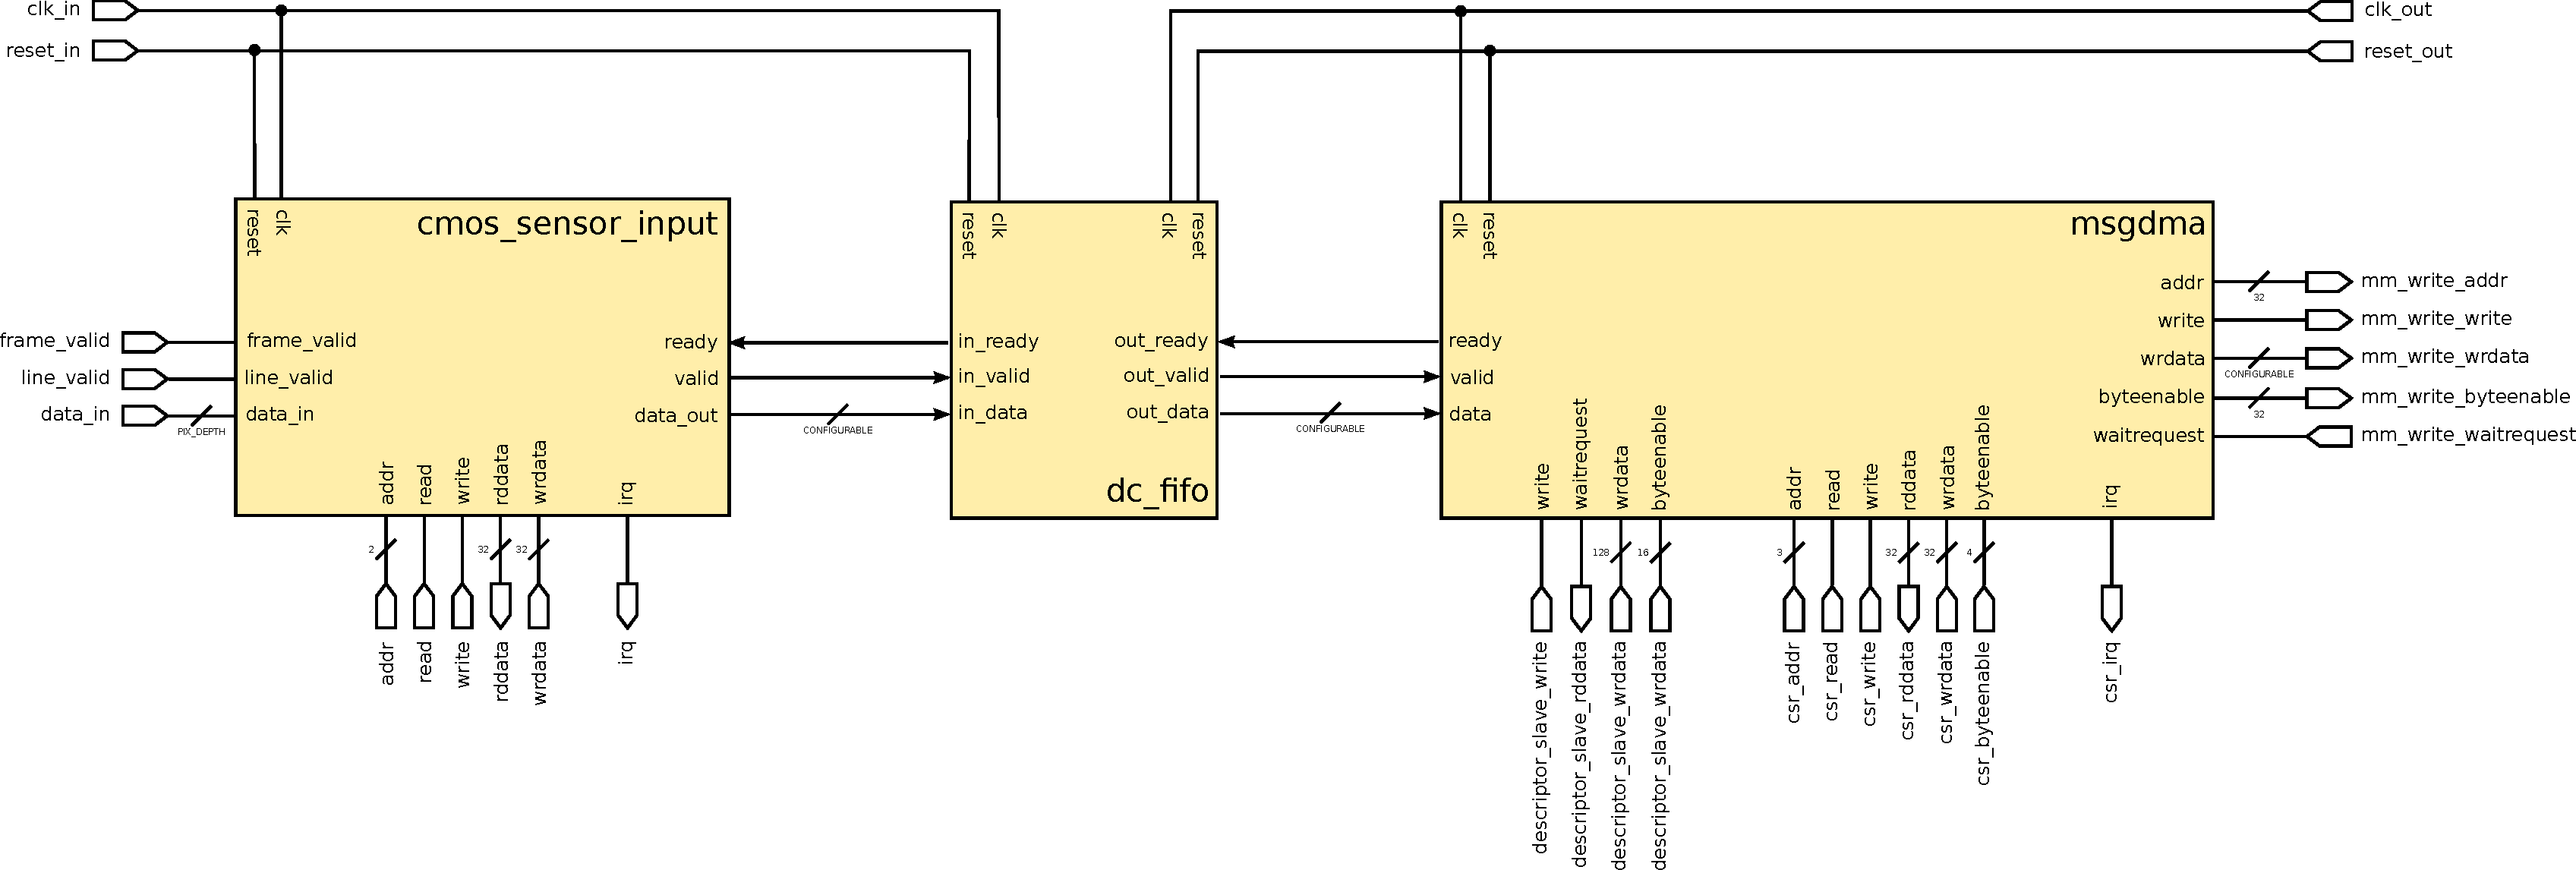
\includegraphics[width=1.0\textwidth]{fig/block_diagram_internal}
    \caption{High-level block diagram.}
    \label{fig:block_diagram_internal}
\end{figure}

\section{Qsys Interface}
Figure~\ref{fig:qsys_gui} shows the Qsys configuration interface for the core.
\begin{figure}[h]
    \centering
    \includegraphics[width=0.9\textwidth]{fig/qsys_gui}
    \caption{Qsys Configuration Interface.}
    \label{fig:qsys_gui}
\end{figure}

It can be configured through 17 parameters, shown in Table~\ref{tab:core_parameters}.

\begin{table}[h]
    \centering
    \makebox[\textwidth][c]{
        \texttt{
            \begin{tabular}{clccc}
                \toprule
                Core                              & Parameter               & Type     & Values                      & Default Value \\
                \midrule
                \multirow{9}{*}{\cmossensorinput} & PIX\_DEPTH              & Positive & 1, 2, 3, ..., 32            & 8             \\
                                                  & SAMPLE\_EDGE            & String   & "RISING", "FALLING"         & "RISING"      \\
                                                  & MAX\_WIDTH              & Positive & 2, 3, 4, ..., 65535         & 1920          \\
                                                  & MAX\_HEIGHT             & Positive & 1, 2, 3, ..., 65535         & 1080          \\
                                                  & OUTPUT\_WIDTH           & Positive & 8, 16, 32, ..., 1024        & 32            \\
                                                  & FIFO\_DEPTH             & Positive & 8, 16, 32, ..., 1024        & 32            \\
                                                  & DEVICE\_FAMILY          & String   & "Cyclone V", "Cyclone IV E" & "Cyclone V"   \\
                                                  & DEBAYER\_ENABLE         & Boolean  & FALSE, TRUE                 & FALSE         \\
                                                  & PACKER\_ENABLE          & Boolean  & FALSE, TRUE                 & FALSE         \\
                \midrule
                \multirow{2}{*}{\dcfifo}          & FIFO\_DEPTH             & Positive & 16, 32, 64, ... , 4096      & 16            \\
                                                  & FIFO\_WIDTH             & Positive & 8, 16, 32, ... , 1024       & 32            \\
                \midrule
                \multirow{6}{*}{\msgdma}          & DATA\_WIDTH             & Positive & 8, 16, 32, ... , 1024       & 32            \\
                                                  & DATA\_FIFO\_DEPTH       & Positive & 16, 32, 64, ... , 4096      & 64            \\
                                                  & DESCRIPTOR\_FIFO\_DEPTH & Positive & 8, 16, 32, ... , 1024       & 8             \\
                                                  & MAX\_BYTE               & Positive & 1KB, 2KB, 4KB, ..., 2GB     & 8MB           \\
                                                  & BURST\_ENABLE           & Boolean  & FALSE, TRUE                 & TRUE          \\
                                                  & MAX\_BURST\_COUNT       & Positive & 2, 4, 8, ... , 1024         & 16            \\
                \bottomrule
            \end{tabular}
        }
    }
    \caption{Qsys parameters.}
    \label{tab:core_parameters}
\end{table}

\section{Results}
\emph{All benchmarks results below were obtained using the default core parameter values shown in Table~\ref{tab:core_parameters}.}

The system was benchmarked on a \texttt{"Cyclone IV E"}-class device, and was able to successfully capture a frame with a resolution of $1920 \times 1080$ pixels under the following timing constraints:

\begin{itemize}
    \itemsep-0.5em
    \item 10 MHz \cmossensorinput clock
    \item \texttt{FRAME\_FRAME\_BLANK = 1}
    \item \texttt{FRAME\_LINE\_BLANK = 0}
    \item \texttt{LINE\_LINE\_BLANK = 1}
    \item \texttt{LINE\_FRAME\_BLANK = 0}
    \item \cmossensorinput \texttt{packer} disabled.
    \item 50 MHz \msgdma clock
\end{itemize}

Note that no camera on the market can actually output frames with such tight frame-frame, frame-line, line-line, and line-frame timings.
The benchmark was rather performed for demonstration purposes to show that the design is able to capture frames under tight constraints.

Furthermore, note that the \cmossensorinput packer was \emph{not} enabled, which would have allowed one to divide the pressure on the memory system by at least a factor of 2. It is recommended to always enable this option, but again, it was left out for demonstration purposes to show the performance of the core.

\newpage

\section{Qsys bugs}
Bug \href{https://www.altera.com/support/support-resources/knowledge-base/solutions/rd05212011_256.html}{rd05212011\_256} may cause issues for the users of the \cmossensoracquisition core.
This bug is caused by the verilog wrapper generated by Qsys to surround the VHDL entity of the \cmossensorinput core contained in this design.

Essentially, the \cmossensorinput core has a few \texttt{Boolean} generic parameters, but the generated verilog code passes \texttt{0} (or \texttt{1}) instead of \texttt{"false"} (or \texttt{"true"}). VHDL being a strongly-typed language, these values are rejected by the synthesizer.

To get around this issue, you must modify the generated verilog wrapper file where the core is instantiated, and replace the boolean parameters by \texttt{"false"} (or \texttt{"true"}) where required.

For example, you would replace the following instantiation code:
\begin{Verbatim}
    cmos_sensor_input #(
        .PIX_DEPTH      (8),
        ...
        .DEBAYER_ENABLE (0),
        .PACKER_ENABLE  (1)
    ) cmos_sensor_input_0 (
        .clk         (clk_in_clk_clk),
        .reset       (rst_controller_reset_out_reset),
        ...
    );
\end{Verbatim}

with the following (changes shown in \textcolor{red}{red}):
\begin{Verbatim}
    cmos_sensor_input #(
        .PIX_DEPTH      (8),
        ...
        .DEBAYER_ENABLE (\textcolor{Red}{"false"}),
        .PACKER_ENABLE  (\textcolor{Red}{"true"})
    ) cmos_sensor_input_0 (
        .clk         (clk_in_clk_clk),
        .reset       (rst_controller_reset_out_reset),
        ...
    );
\end{Verbatim}

Remember to keep the quotes, as they are \emph{necessary}.

\end{document}
